\documentclass[12pt]{article}

\usepackage[top=2.54cm, bottom=2.54cm, left=2.54cm, right=2.54cm]{geometry}
\usepackage{amsfonts}
\usepackage{amsmath}
\usepackage{amsthm}
\usepackage{amsbsy}
\usepackage{graphicx}
\usepackage{parskip}
\usepackage{subcaption}
\usepackage{url}

\newcommand\N{\ensuremath{\mathbb{N}}}
\newcommand\R{\ensuremath{\mathbb{R}}}
\newcommand\Z{\ensuremath{\mathbb{Z}}}
\renewcommand\O{\ensuremath{\emptyset}}

\pagestyle{plain}
\title{Journal for Math153 (ODEs)}
\author{Jonathan Conroy}
\date{Fall 2021}
\begin{document}
\maketitle
\tableofcontents
\newpage
\section{What is Mathematics? (9/9/21)}
I read the New Yorker article linked in the prompt. This article ends with the quote ``In Book 7 of the Republic, Plato has Socrates say that mathematicians are people who dream that they are awake.'' Having taken an (introductory) course on the Republic, I found this to be a really interesting statement and attempted to dig into this idea further.

The full quote, found in Book 7 (533c-d), is as follows:
\begin{quote}
The [arts] which we said did in some sort lay hold on reality — geometry and the studies that accompany it — are, as we see, dreaming about being, but the clear waking vision of it is impossible for them as long as they leave the assumptions which they employ undisturbed and cannot give any account of them. For where the starting-point is something that the reasoner does not know, and the conclusion and all that intervenes is a tissue of things not really known, what possibility is there that assent in such cases can ever be converted into true knowledge or science?
\end{quote}

Plato uses the metaphor of the dream as something which partially reflects (and is an imperfect image of) reality but is not reality itself. By saying that the mathematician is a dreamer who believes that they are awake, Plato claims that the mathematician believes that they possess true knowledge but that in fact they do not. The reason for this, Plato argues, is that mathematical theorems can be constructed independent from the real world, and mathematicians concern themselves only with the consequences of unquestioned axioms. So long as those axioms remain unquestioned, the mathematician can never have ``true'' knowledge.

This is a fascinating idea in the context of our discussion last class. Many definitions people proposed (at least, the ones that I found most convincing) seemed to fall along the lines of ``math is organized abstraction'' or ``math is the study of patterns.'' At first glance, these seem like they could be independent of the real world. But what does math abstract \textit{from}? Where do people look to find patterns that they then attempt to abstract and analyze mathematically? One could attempt to generalize existing math, but often the real world is used as a source of inspiration. Plato almost seems to be suggesting that this is a good thing - mathematicians \textit{should} examine and reexamine the real world and attempt to develop theories that are consistent with and motivated by it.

\textbf{Sources}:
\begin{enumerate}
    \item New Yorker article: \url{https://www.newyorker.com/culture/culture-desk/what-is-mathematics}
    \item Paper discussing Plato's quote: \url{https://orb.binghamton.edu/cgi/viewcontent.cgi?article=1034&context=sagp}
    \item Translation of the Republic: \url{http://www.perseus.tufts.edu/hopper/text?doc=Perseus%3Atext%3A1999.01.0168%3Abook%3D7%3Apage%3D533}
\end{enumerate}

\newpage

\section{Modeling Herd Immunity}
\subsection{SIR $\alpha$ Parameter, Part I (9/14/21)}
The SIR model presented in class has the following form:
$$S_{k+1} = S_k - \alpha S_k I_k$$
$$I_{k+1} = \alpha S_k I_k$$
$$R_{k+1} = I_k$$
where $S_k$, $I_k$, and $R_k$ denote the number of susceptible, infected, and recovered/dead agents. It was mentioned in class that the $\alpha$ parameter can be thought of similarly to the ``probability of transmission'' parameter from an earlier model.  However, $\alpha$ cannot exactly be the probability that an infected person infects a susceptible person: if $\alpha = 1$ (a valid probability) and $I_0$ starts off as $2$ (which, given that it is small, seems like a reasonable thing to want to allow), then $S_{1} = S_0 - 2 S_0 < 0$. This is completely nonsensical, of course.

Given that $\alpha$ is not the probability of transmission, it is natural to ask how it is \textit{related} to the probability of transmission. 

A natural model of infection is to say that $S_{k+1} = S_{k} - (\text{probability of one person becoming infected}) S_{k}$. We can calculate the probability of a single susceptible person becoming infected as follows:

Let $p$ be the probability of a single infected person infecting a single susceptible person. Then:

\begin{align*}
P(\text{person becomes infected}) &= 1 - P(\text{person is not infected})\\
&= 1 - [P(\text{person is not infected by A}) \cdot P(\text{person is not infected by B}) \cdot \hdots]\\
&= 1 - (1-p)^{I_k}
\end{align*}

If this is the same model as the SIR model, then $\alpha S_k$ must be the probability that a single susceptible person becomes infected in one timestep. Thus $\alpha = \frac{1 - (1-p)^{I_k}}{I_k}$. This does not seem promising - the relationship between $\alpha$ and $p$ depends on $S_k$ and $I_k$, the number of \textit{currently} susceptible people, and is not constant.

\subsection{SIR $\alpha$ Parameter, Part II (9/16/21)}
In the previous journal entry, I proposed another model based on the probability $p$ for a person to be infected by one other person. This ``$p$-based'' model was the same as the SIR model except that 
$$S_{k+1} = S_{k} - (1 - (1-p)^{I_k}) S_{k}$$
and similarly
$$I_{k+1} = (1 - (1-p)^{I_k}) S_{k}$$

There was no nice relation between the SIR model and the other $p$-based model. The reason for this seems to be the fact that $P(A \cup B) \neq P(A) + P(B)$ in general. In other words, the probability that a person is infected is when there are 2 infected people if \textit{not} exactly twice the probability that they are infected when there is only 1 infected person.

A natural question is - how bad is this approximation? Does the SIR model capture roughly the same information as the $p$-based model, or does the assumption that $P(A \cup B) = P(A) + P(B)$ result in a significantly different infection curve?

I coded the SIR model and the $p$-based model in Python. I chose $\alpha$, $S_0$, and $I_0$ values that resulted in an infection curve that looked ``normal'': $\alpha = 0.00013$, $S_0 = 9999$, and $I_0 = 1$ so that $\alpha S_0 \approx 1.3$ is slightly larger than 1.

I then attempted to find the best $p$ so that SIR simulation and the $p$-based simulation produced similar results. To do this, we need some way to measure goodness-of-fit. Rather arbitrarily, I chose to measure the distance between two simulation results $(S_k, I_k, R_k)$ and $(S'_k, I'_k, R'_k)$ by $\sum_k \lvert I_k - I'_k \rvert$. The \texttt{scipy.optimize} package was used to find the value of $p$ that minimizes this distance. See Figure 1(a). See Figure 2(b) and 2(c) for simulations of other values of $\alpha$.

Surprisingly, the two models appear to produce very similar results! Further, the value of $p$ that minimizes the distance is \textit{very} close to $\alpha$ (specifically, $p = 0.00013042$). I am not entirely sure why this is. Perhaps the relationship $\alpha = \frac{1 - (1-p)^{I_k}}{I_k}$ simplifies to something nicer?

\begin{figure}[t!]
\centering
\begin{subfigure}[t]{0.3\textwidth}
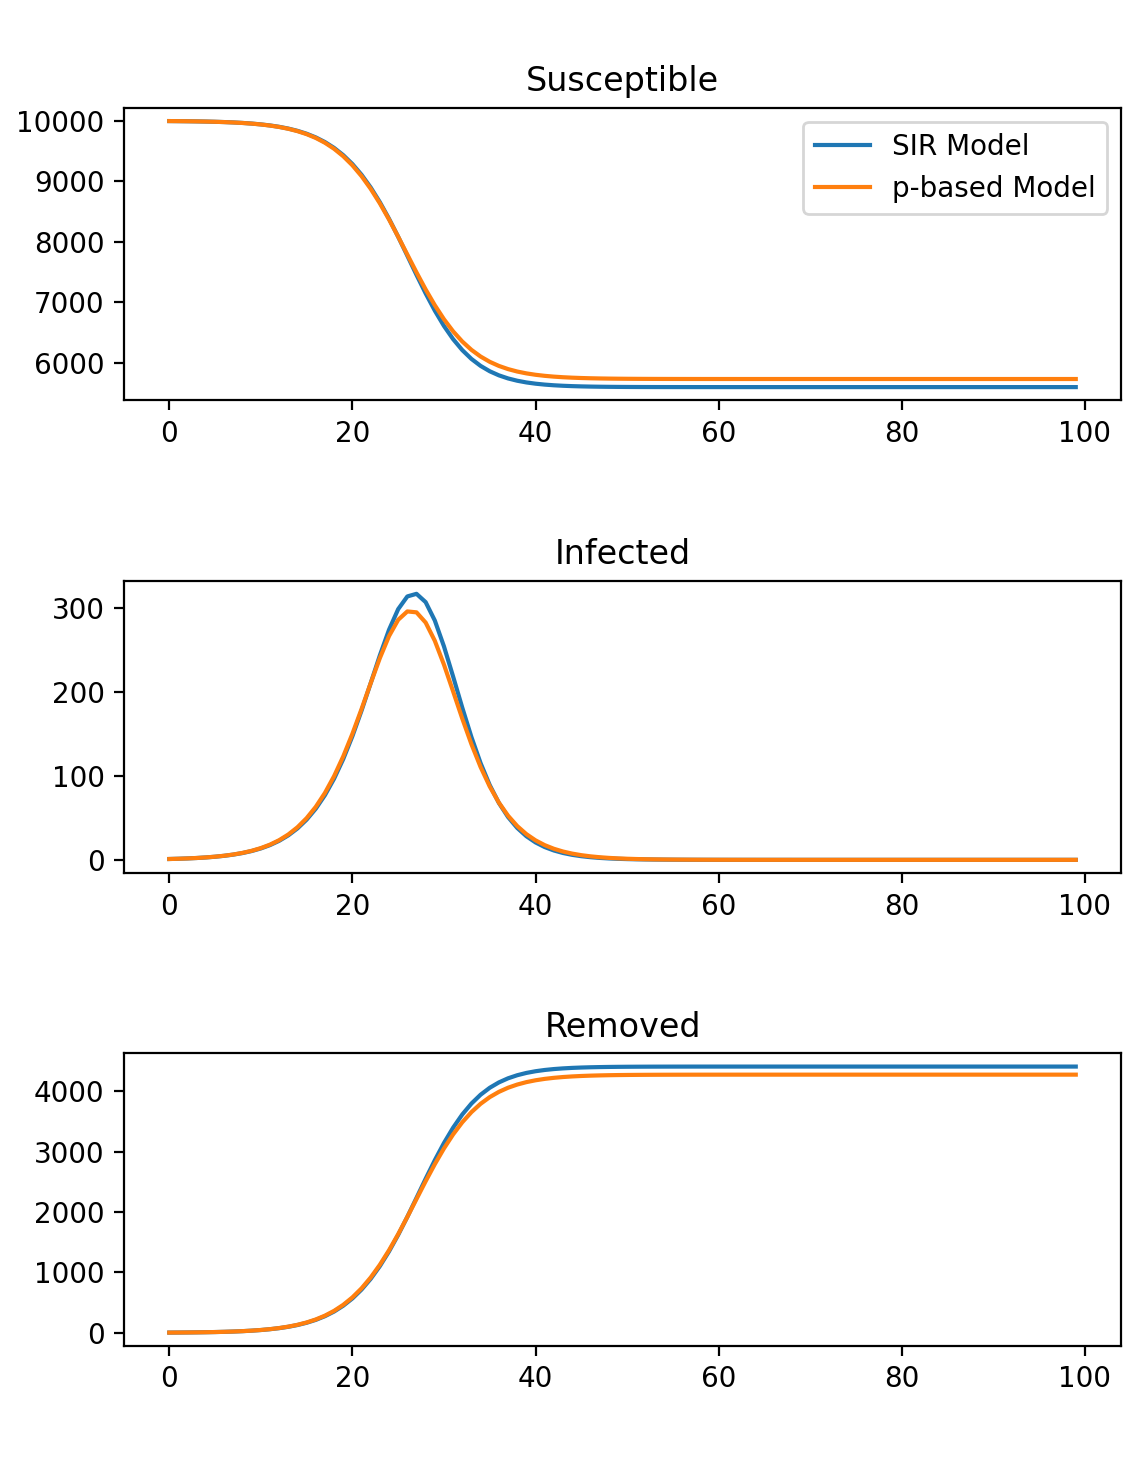
\includegraphics[width=\textwidth]{sir_comparison_13.png}
\caption{$\alpha = 0.00013$ and $p = 0.00013042$}
\end{subfigure}
~
\begin{subfigure}[t]{0.3\textwidth}
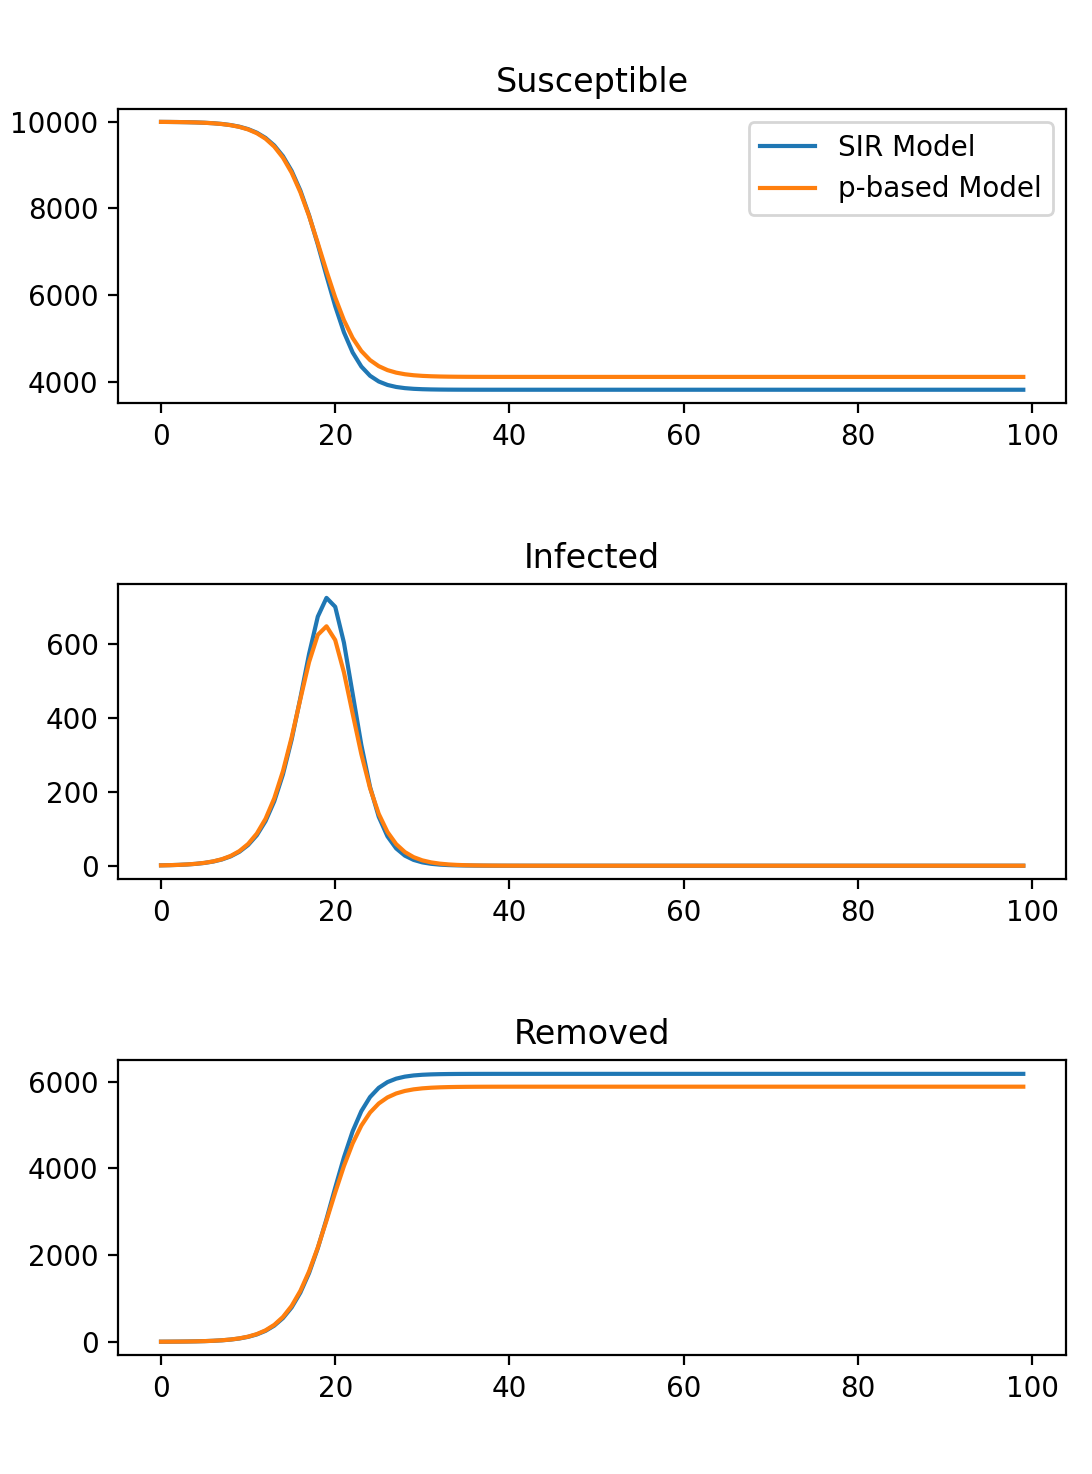
\includegraphics[width=\textwidth]{sir_comparison_15.png}
\caption{$\alpha = 0.00015$ and $p = 0.00015091$}
\end{subfigure}
~
\begin{subfigure}[t]{0.3\textwidth}
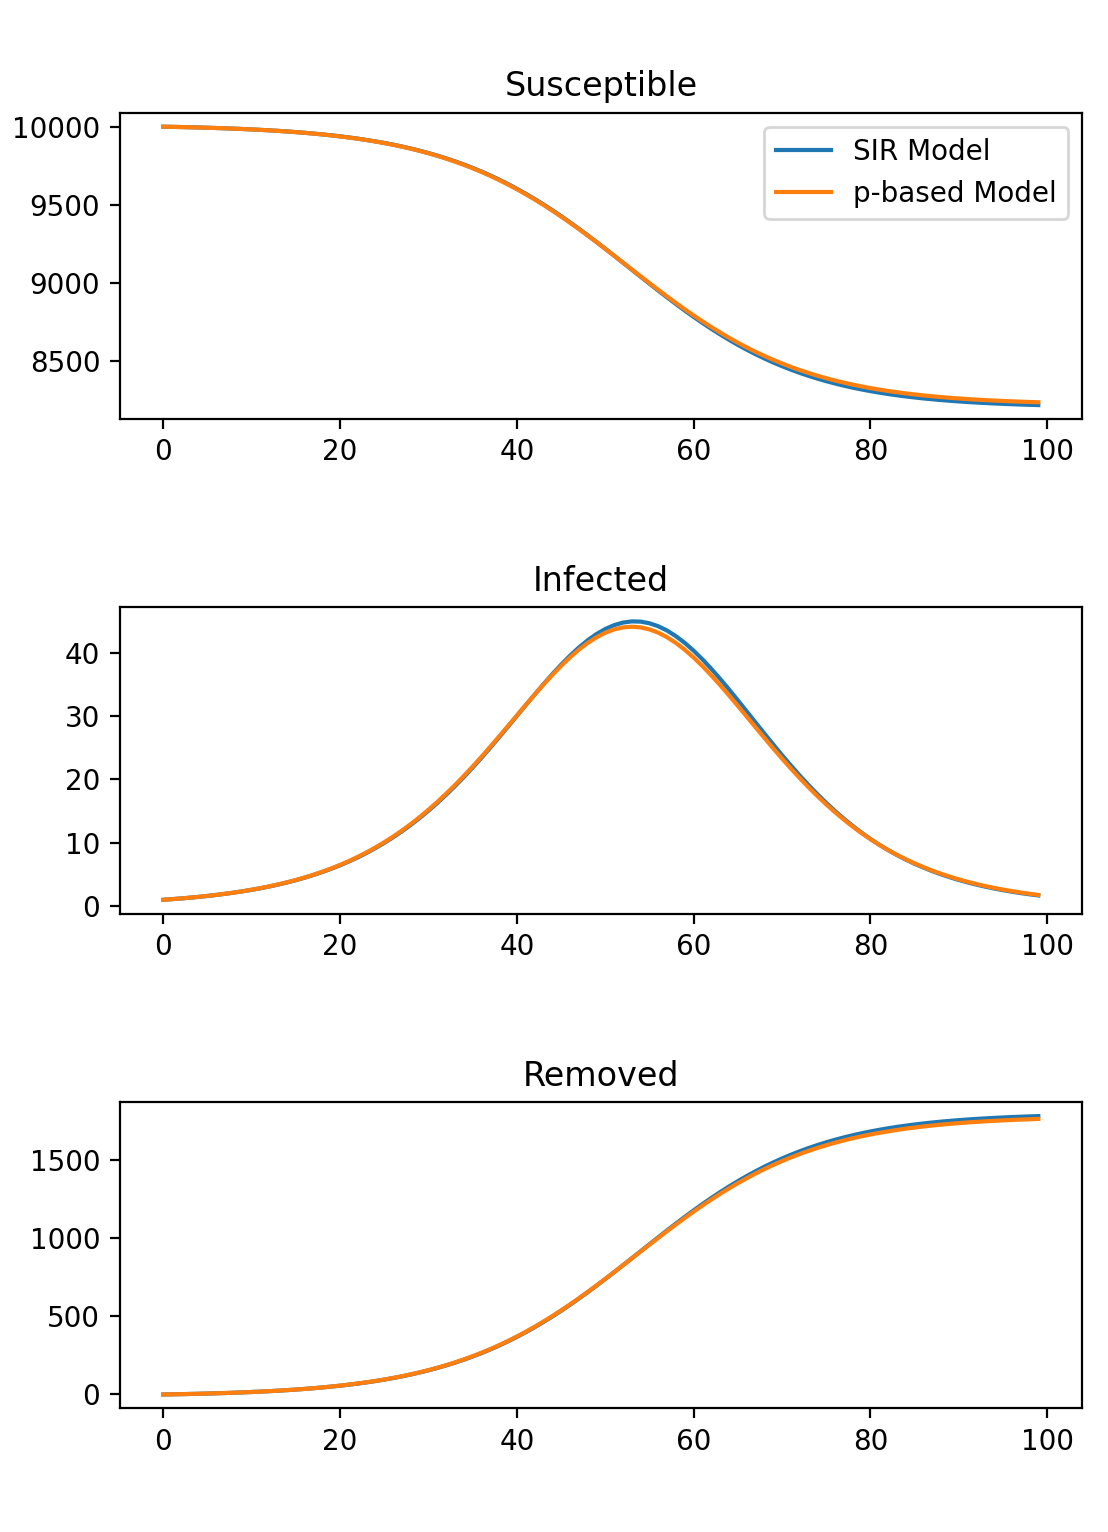
\includegraphics[width=\textwidth]{sir_comparison_11.png}
\caption{$\alpha = 0.00011$ and $p = 0.00011007$}
\end{subfigure}
\end{figure}

\newpage

\subsection{SIR $\alpha$ Parameter, Part III (9/21/21)}
After a discussion with Prof. Borgers, I corrected a minor mistake in the model proposed above: the denominator of $\alpha = \frac{1 - (1-p)^{I_k}}{I_k}$ is $I_k$, not $S_k$ as originally written. Prof. Borgers also suggested that this quantity is approximately a constant for small values of $n$, if we assume that $p$ is very small. This entry attempts to spell out the argument somewhat explicitly, though I am \textit{very} informal with ``approximately equal to''.

We want to expand $\alpha = f(x) = \frac{1 - (1-p)^{x}}{x}$ as a Taylor series around $x = 0$. However, this would be undefined: instead, we take the limit as $x$ approaches $0$.\\

\textit{Claim 1: $\lim_{x \to 0} \frac{1-(1-p)^x}{x} = -\ln(1-p) \approx p$ for small values of $p$}
\begin{proof}
Apply L'Hopital's rule:
$$\lim_{x \to 0} \frac{1-(1-p)^x}{x} = \lim_{x \to 0} \frac{-1 \cdot \ln(1-p) \cdot (1-p)^x}{1} = - \ln(1-p)$$
Because $p$ is small, we can approximate this by expanding $-\ln(1-p)$ as a Taylor series around $p = 0$.
$$-\ln(1-p) = 0 + \frac{1}{1-p}p + \hdots \approx \frac{p}{1-p}$$
Notice that $\frac{1}{1-p} = 1 + p + p^2 + p^3 + \hdots$ for $p < 1$, so $$-\ln(1-p) \approx p + p^2 + \hdots \approx p$$ for small $p$. (Note that this is a very informal argument)
\end{proof}


\textit{Claim 2: $\lim_{x \to 0} \frac{d}{dx} \frac{1-(1-p)^x}{x} = \frac{-\ln^2 (1-p)}{2} \approx 0 \approx p$ for small values of $p$}
\begin{proof}
By the quotient rule for derivatives:
\begin{align*}
\frac{d}{dx} \frac{1 - (1-p)^x}{x} &= \frac{x(-\ln(1-p) \cdot (1-p)^x) - (1-(1-p)^x)}{x^2}\\
&= \frac{-\ln(1-p) \cdot x(1-p)^x + (1-p)^x - 1}{
x^2}\\
&= \frac{(-\ln(1-p) \cdot x + 1 )(1-p)^x - 1}{x^2}
\end{align*}
Taking the limit as $x$ approaches $0$ and repeatedly applying L'Hopital's rule, we find:
\begin{align*}
\lim_{x \to 0}
\frac{(-\ln(1-p) \cdot x + 1 )(1-p)^x - 1}{x^2}
&=\lim_{x \to 0} \frac{(-\ln(1-p) \cdot x + 1)\cdot \ln(1-p) \cdot (1-p)^x - \ln(1-p) \cdot (1-p)^x}{2x}\\
&= \lim_{x \to 0}\frac{(-\ln(1-p) \cdot x + 1)\cdot \ln(1-p) \cdot (1-p)^x - \ln(1-p) \cdot (1-p)^x}{2x}\\
&= \lim_{x \to 0}\frac{-\ln^2(1-p) \cdot x \cdot (1-p)^x}{2x}\\
&= \lim_{x \to 0} \frac{-\ln^2(1-p) \cdot [x (\ln(1-p) \cdot (1-p)^x) + (1-p)^x]}{2}\\
&= \lim_{x \to 0} \frac{-\ln^3(1-p) \cdot x \cdot (1-p)^x - \ln^2(1-p) \cdot (1-p)^x}{2}\\
&= \frac{-\ln^2(1-p)}{2}
\end{align*}
When $p$ is small, $1 - p$ will be close to $1$ and so $\frac{-\ln^2(1-p)}{2} \approx 0$. 
\end{proof}

This means that the Taylor series expansion of $\frac{1-(1-p)^x}{x}$ near $x = 0$ is (for small $p$) approximately:
$$\frac{1-(1-p)^x}{x} \approx p + 0 \cdot x + [\text{higher order terms...}] \approx p$$.

\subsection{Non-Uniqueness of Initial Value Problems (9/23/21)}
This entry responds the first prompt posed by Prof. Borgers in the \texttt{09\_23\_things\_to\_think\_about.pdf} document. We proved in class that under certain conditions, initial value problems have unique solutions. Consider the problem:
$$\frac{dx}{dt} = x^{1/3} \quad\quad\quad\quad x(0) = 0$$
$x^{1/3}$ is not differentiable at $x = 0$, so it does not satisfy the conditions from class.

We apply separation of variables to find one solution:
\begin{align*}
\frac{dx}{dt} &= x^{1/3}\\
x^{-\frac{1}{3}} \frac{dx}{dt} &= 1\\
\end{align*}
Notice that the left-hand side is the derivative (with respect to $t$) of $\frac{3}{2}x^\frac{2}{3}$. Thus,
\begin{align*}
\frac{d}{dt} \frac{3}{2}x^\frac{2}{3} &= 1\\
\frac{d}{dt} \int_0^t \frac{3}{2}x^\frac{2}{3} ds &= \int_0^t 1 ds\\
\frac{3}{2}x^\frac{2}{3} &= t + C\\
x &= \left(\frac{2}{3}t + \frac{2}{3}C \right)^{\frac{3}{2}}
\end{align*}
As $x(0) = 0$, $0 = \left(\frac{2}{3}C \right)^{\frac{3}{2}}$ and so $C = 0$. Thus, one solution is $x(t) = \left(\frac{2}{3}t\right)^{3/2}$\\

In fact, there are infinitely many solutions. For any real number $t_0 \ge 0$, the following is a solution:
$$x_{t_0}(t) = \begin{cases}
0 & \text{if $t < t_0$}\\
\left(\frac{2}{3}t\right)^{3/2} & \text{otherwise}
\end{cases}$$
Notice that 

$$\frac{d}{dt} x_{t_0}(t) \quad = \quad \begin{cases}
0 & \text{if $t < t_0$}\\
\frac{3}{2} \cdot \frac{2}{3} \cdot \left(\frac{2}{3}t\right)^{1/2}  & \text{otherwise}
\end{cases}
\quad = \quad
\begin{cases}
0 & \text{if $t < t_0$}\\
\left(\frac{3}{2}t\right)^{1/2} & \text{otherwise}
\end{cases}$$
Further:

$$x_{t_0}(t)^{1/3}
\quad = \quad
\begin{cases}
0 & \text{if $t < t_0$}\\
\left(\frac{2}{3}t\right)^{3/2 \cdot 1/3} & \text{otherwise}
\end{cases}
\quad = \quad
\begin{cases}
0 & \text{if $t < t_0$}\\
\left(\frac{2}{3}t\right)^{1/2} & \text{otherwise}
\end{cases}$$
Thus, every $x_{t_0}(t)$ satisfies the differential equation. As $t_0 \ge 0$, $x_{t_0}(0) = 0$.


\end{document}
